\documentclass[11pt,letter]{article}
% \include{macro-file}

\def\mainroot{ell_1}

%%%%%% Margins and spacing
\usepackage[top=1in, bottom=1in, left=1in, right=1in]{geometry}
\usepackage{algorithm}
\usepackage{amsmath}
\usepackage{url}
\usepackage{caption}
\usepackage[compact]{titlesec}
%\usepackage{bm}
\usepackage{txfonts} %\usepackage{times}
\usepackage{color}
\usepackage{tikz}
\usetikzlibrary{calc}
\usepackage{cancel}
\usepackage{soul}
\usepackage{graphicx}
\usepackage{caption}
\usepackage{subcaption}
\usepackage{algpseudocode}
\usepackage{listings}

\usepackage{sidecap}
\sidecaptionvpos{figure}{c}

\usepackage{enumitem}
\setlist{nolistsep}

\definecolor{commentcolor}{HTML}{FF3300}
\definecolor{keywordcolor}{HTML}{0000FF}
\definecolor{idcolor}{HTML}{000099}

%\setcounter{MaxMatrixCols}{20}

\newcommand\mjsnote[1]{{\bf [#1 -mjs]}}

\newcommand{\meas}{{\mathbf \mu}}
\newcommand{\tightpgh}[1]{\vskip 3pt\noindent\textbf{#1}}
\newcommand{\signalw}{{\mathbf w}}
\newcommand{\signalx}{{\mathbf x}}
\newcommand{\signaly}{{\mathbf y}}
\newcommand{\signalz}{{\mathbf z}}

%\expandafter\def\expandafter\normalsize\expandafter{%
%    \normalsize
%    \setlength\abovedisplayskip{2pt}
%    \setlength\belowdisplayskip{2pt}
%    \setlength\abovedisplayshortskip{0pt}
%    \setlength\belowdisplayshortskip{0pt}
%}\makeatother
%
%\renewcommand\floatpagefraction{.9}
%\renewcommand\topfraction{.9}
%\renewcommand\bottomfraction{.9}
%\renewcommand\textfraction{.1}   
%\setlength{\textfloatsep}{10pt plus 1.0pt minus 2.0pt}

% Jian \DeclareMathOperator*{\median}{median}
\newcommand{\mb}{\ensuremath\mathbf}
\newcommand{\F}{\ensuremath\mathbb{F}}

\title{CSE537 Assignment-1 Report: Peg Solitaire}
\author{
%\alignauthor
Remy Oukaour \\
       {\small SBU ID: 107122849}\\
       {\small \texttt{remy.oukaour@gmail.com }}
%\alignauthor
\and
Jian Yang \\
       {\small SBU ID: 110168771}\\
       {\small \texttt{jian.yang.1@stonybrook.edu }}
%\alignauthor
}
\date{}


\raggedbottom

\begin{document}
\maketitle

\begin{abstract}
This is a report for the assignment 1 in course CSE537 Artificial Intelligence. Assignment 1 required to implement the ID-DFS( iterative deepening depth-first search) and two different heuristic A* methods. \\
In this report, we would discuss the implementation details, and we also compared the six solutions, including the ID-DFS method, six A* methods and one baseline.
\end{abstract}

% \thispagestyle{empty}
% \newpage
% \addtocounter{page}{-1}

\section{Introduction}
TODO: write the introduction

\section {Implementation}\label{sec:var}
\subsection {Data Structure Optimazation}
\subsubsection {pegSolitaire}
The original data structure to present pegSolitaire is a single state node to present a node. For the implementation for A* and the purpose to make the routine more clear, we separated the game wrapper and the game state to two different classes, the first one is the class \(game\) and the second one is the class \(gameNode\).
\subsubsection {gameState}
The original data structure to save game state in given framework was a 2-dimensional integer array. The indexing to every single entry required two indexes, one is the column and another is the row. To simplify this, we flattened the array to 1-dimensional. According to that, the size of the array is 49, and we mapped the original entries to 1-dimenstional array by \(new\_pos = old\_pos[0] \times 7 + old\_pos[1]\) where \(new\_pos\) is the index in 1-dimensional array and \(old\_pos\) is the indexes tuple in 2-dimensional array. 

\subsection {Required Implementation}
There are four required implementation in file pegSolitaireUtils.py: \\
\begin{enumerate}
\item is\_corner(self, pos):
\lstset{language=Python,
                basicstyle=\ttfamily,
                showstringspaces=false,
                keywordstyle=\color{keywordcolor}\ttfamily,
                identifierstyle=\color{idcolor}\ttfamily,
                stringstyle=\color{red}\ttfamily,
                commentstyle=\color{commentcolor}\ttfamily,
                numberstyle=\color{keywordcolor}\ttfamily,
                morecomment=[l][\color{magenta}]{\#}
}

\begin{lstlisting}[frame=single]  % Start your code-block

def is_corner(self, pos):
    """
        Return whether a position is a corner/wall,
        i.e. not a hole or peg.
    """
    return 0 <= pos < 49 and self.state[pos] != -1
\end{lstlisting}

In implementation, we used another function \(\_\_getitem\_\_(self, pos)\) instead: \\
\lstset{language=Python,
                basicstyle=\ttfamily,
                showstringspaces=false,
                keywordstyle=\color{keywordcolor}\ttfamily,
                identifierstyle=\color{idcolor}\ttfamily,
                stringstyle=\color{red}\ttfamily,
                commentstyle=\color{commentcolor}\ttfamily,
                numberstyle=\color{keywordcolor}\ttfamily,
                morecomment=[l][\color{magenta}]{\#}
}

\begin{lstlisting}[frame=single]  % Start your code-block

def __getitem__(self, pos):
    """
    node[pos] is bounds-checked shorthand for node.state[pos].
    """
    return self.state[pos] if 0 <= pos < 49 else -1
\end{lstlisting}

\item \(is\_validMove(self, oldPos, direction):\)
\lstset{language=Python,
                basicstyle=\ttfamily,
                showstringspaces=false,
                keywordstyle=\color{keywordcolor}\ttfamily,
                identifierstyle=\color{idcolor}\ttfamily,
                stringstyle=\color{red}\ttfamily,
                commentstyle=\color{commentcolor}\ttfamily,
                numberstyle=\color{keywordcolor}\ttfamily,
                morecomment=[l][\color{magenta}]{\#}
}

\begin{lstlisting}[frame=single]  % Start your code-block

def is_validMove(self, oldPos, direction):
    """
    Return whether it is valid to move a peg from a given position
    in a given direction. The position must have a peg, the 
    destination must be empty, and the intermediate position
    must have another peg.
    """
    # Since self.getNextPosition and self.__getitem__ are
    # bounds-checked.
    # the self.is_corner check is redundant, so I commented it out
    #########################################
    # DONT change Things in here
    # In this we have got the next peg position and
    # below lines check for if the new move is a corner
    #newPos = self.getNextPosition(oldPos, direction)
    #if self.is_corner(newPos):
    #	return False
    ########################################
    # YOU HAVE TO MAKE CHANGES BELOW THIS
    # check for cases like:
    # if new move is already occupied
    # or new move is outside peg Board
    # Remove next line according to your convenience
    midPos = self.getNextPosition(oldPos, direction)
    newPos = self.getNextPosition(midPos, direction)
    # 1 is a peg, and 0 is a hole
    # Since oldPos is valid, don't use bounds-checked indexing
    # for it
    return (self.state[oldPos] == self[midPos] == 1 and\
               self[newPos] == 0)
\end{lstlisting}
\item getNextPosition(self, oldPos, direction):
\lstset{language=Python,
                basicstyle=\ttfamily,
                showstringspaces=false,
                keywordstyle=\color{keywordcolor}\ttfamily,
                identifierstyle=\color{idcolor}\ttfamily,
                stringstyle=\color{red}\ttfamily,
                commentstyle=\color{commentcolor}\ttfamily,
                numberstyle=\color{keywordcolor}\ttfamily,
                morecomment=[l][\color{magenta}]{\#}
}

\begin{lstlisting}[frame=single]  % Start your code-block

@staticmethod
def getNextPosition(oldPos, direction):
    """
    Return the new position after moving in the given direction
    (7 is north/up, 1 is east/right, -7 is south/down, and -1 is
    west/left).
    Invalid movements outside the bounds of the board will return
    positions such that is_corner(position) returns True.
    """
    newPos = oldPos + direction
    # If direction is 7 or -7 (changing rows), newPos is already
    # correct
    return (newPos if direction == 7 or direction == -7 or
    # If direction is 1 or -1 (changing columns), the row should
    # not change
        newPos // 7 == oldPos // 7 else -1)
\end{lstlisting}
\item getNextState(self, oldPos, direction):
\lstset{language=Python,
                basicstyle=\ttfamily,
                showstringspaces=false,
                keywordstyle=\color{keywordcolor}\ttfamily,
                identifierstyle=\color{idcolor}\ttfamily,
                stringstyle=\color{red}\ttfamily,
                commentstyle=\color{commentcolor}\ttfamily,
                numberstyle=\color{keywordcolor}\ttfamily,
                morecomment=[l][\color{magenta}]{\#}
}

\begin{lstlisting}[frame=single]  % Start your code-block

def getNextState(self, oldPos, dir, pegSol):
    """
    Return a child node of the current one, created by a given
    valid move.
    The given game has its count of expanded nodes incremented.
    """
    ###############################################
    # DONT Change Things in here
    pegSol.nodesExpanded += 1
    if not self.is_validMove(oldPos, dir):
        print "Error, You are not checking for valid move"
        exit(0)
    ###############################################
    # YOU HAVE TO MAKE CHANGES BELOW THIS
    # Update the gameState after moving peg
    # eg: remove crossed over pegs by replacing it's
    # position in gameState by 0
    # and updating new peg position as 1
    midPos = self.getNextPosition(oldPos, dir)
    newPos = self.getNextPosition(midPos, dir)
    # x[:] makes a copy of x (necessary to avoid mutating
    # self.state when updating childState)
    childState = self.state[:]
    childState[oldPos] = 0 # The peg moves from here, leaving a hole
    childState[midPos] = 0 # The jumped-over peg is removed
    childState[newPos] = 1 # The peg moves to this hole
    # Convert positions back into pairs for printing
    childTrace = self.trace + [(oldPos // 7, oldPos % 7), \
                        (newPos // 7, newPos % 7)]
    return gameNode(childState, childTrace, self.pegCount - 1,\
              self.heuristic)
\end{lstlisting}
\end{enumerate}

\subsection {Implementation of methods}
\subsubsection {ID-DFS}

\subsubsection {A* with heuristic method 1}
\lstset{language=Python,
                basicstyle=\ttfamily,
                showstringspaces=false,
                keywordstyle=\color{keywordcolor}\ttfamily,
                identifierstyle=\color{idcolor}\ttfamily,
                stringstyle=\color{red}\ttfamily,
                commentstyle=\color{commentcolor}\ttfamily,
                numberstyle=\color{keywordcolor}\ttfamily,
                morecomment=[l][\color{magenta}]{\#}
}

\begin{lstlisting}[frame=single]  % Start your code-block

	distances = [
		5, 4, 3, 2, 3, 4, 5,
		4, 3, 2, 1, 2, 3, 4,
		3, 2, 1, 0, 1, 2, 3,
		2, 1, 0, 1, 0, 1, 2,
		3, 2, 1, 0, 1, 2, 3,
		4, 3, 2, 1, 2, 3, 4,
		5, 4, 3, 2, 3, 4, 5
	]
\end{lstlisting}
\subsubsection {A* with heuristic method 2}
\lstset{language=Python,
                basicstyle=\ttfamily,
                showstringspaces=false,
                keywordstyle=\color{keywordcolor}\ttfamily,
                identifierstyle=\color{idcolor}\ttfamily,
                stringstyle=\color{red}\ttfamily,
                commentstyle=\color{commentcolor}\ttfamily,
                numberstyle=\color{keywordcolor}\ttfamily,
                morecomment=[l][\color{magenta}]{\#}
}

\begin{lstlisting}[frame=single]  % Start your code-block

	# difficulties = [
	# 	0, 0, 4, 0, 4, 0, 0,
	# 	0, 0, 0, 0, 0, 0, 0,
	# 	4, 0, 3, 0, 3, 0, 4,
	# 	0, 0, 0, 1, 0, 0, 0,
	# 	4, 0, 3, 0, 3, 0, 4,
	# 	0, 0, 0, 0, 0, 0, 0,
	# 	0, 0, 4, 0, 4, 0, 0,
	# ]
\end{lstlisting}
\subsubsection {A* with heuristic method 3}
\lstset{language=Python,
                basicstyle=\ttfamily,
                showstringspaces=false,
                keywordstyle=\color{keywordcolor}\ttfamily,
                identifierstyle=\color{idcolor}\ttfamily,
                stringstyle=\color{red}\ttfamily,
                commentstyle=\color{commentcolor}\ttfamily,
                numberstyle=\color{keywordcolor}\ttfamily,
                morecomment=[l][\color{magenta}]{\#}
}

\begin{lstlisting}[frame=single]  % Start your code-block

def heuristicThree(node):
	state = node.state
	# Count the number of dangling pegs
	num_dangling = 0
	for i in xrange(49):
		if state[i] != 1: continue
		for direction in [7, 1, -7, -1]:
			if node[i + direction] == 1:
				break
		else:
			num_dangling += 1
	return node.pegCount * 2 + num_dangling
\end{lstlisting}
\subsubsection {A* with heuristic method 4}
\lstset{language=Python,
                basicstyle=\ttfamily,
                showstringspaces=false,
                keywordstyle=\color{keywordcolor}\ttfamily,
                identifierstyle=\color{idcolor}\ttfamily,
                stringstyle=\color{red}\ttfamily,
                commentstyle=\color{commentcolor}\ttfamily,
                numberstyle=\color{keywordcolor}\ttfamily,
                morecomment=[l][\color{magenta}]{\#}
}

\begin{lstlisting}[frame=single]  % Start your code-block

	# corners = [
	# 	0, 0, 1, 1, 1, 0, 0,
	# 	0, 0, 1, 1, 1, 0, 0,
	# 	1, 1, 0, 0, 0, 1, 1,
	# 	1, 1, 0, 0, 0, 1, 1,
	# 	1, 1, 0, 0, 0, 1, 1,
	# 	0, 0, 1, 1, 1, 0, 0,
	# 	0, 0, 1, 1, 1, 0, 0,
	# ]
\end{lstlisting}
\subsubsection {Baseline for A*}
We used the number of left pegs to be the cost function for a baseline methods.

\subsubsection {A* with heuristic method mixed from 2 and 4}
\lstset{language=Python,
                basicstyle=\ttfamily,
                showstringspaces=false,
                keywordstyle=\color{keywordcolor}\ttfamily,
                identifierstyle=\color{idcolor}\ttfamily,
                stringstyle=\color{red}\ttfamily,
                commentstyle=\color{commentcolor}\ttfamily,
                numberstyle=\color{keywordcolor}\ttfamily,
                morecomment=[l][\color{magenta}]{\#}
}

\begin{lstlisting}[frame=single]  % Start your code-block

	difficulties = [
		0, 0, 4, 1, 4, 0, 0,
		0, 0, 1, 1, 1, 0, 0,
		4, 1, 2, 0, 2, 1, 4,
		1, 1, 0, 1, 0, 1, 1,
		4, 1, 2, 0, 2, 1, 4,
		0, 0, 1, 1, 1, 0, 0,
		0, 0, 4, 1, 4, 0, 0,
	]
\end{lstlisting}

\subsubsection {Other abandoned methods}
We also tried Manhattan distances but this cost function doesn't work well as the above methods we used. So we didn't include it in the following performance disucssion.

\subsection {Other Optimization for Performance}

\section {Benchmark}
\subsection {Manual Tests}
We have written 10 manual cases from impossible cases to extreme cases.
\subsection {Random Tests}
For test purpose, we implemented one random generator to generate a game board status. The idea is, based on the final state, we would randomly generate a valid backward move based on current board and apply the move and repeat this for random steps. \\
The pseudocode is:
\begin{algorithm}                      % enter the algorithm environment
\caption{Random Test generator}          % give the algorithm a caption
\label{random_alg}                           % and a label for \ref{} commands later in the document
\begin{algorithmic} [1]                   % enter the algorithmic environment
    \State {$num\_step \gets$  a random number between 1 and 33 }
    \State {$board\_state \gets$ initialized board state with only one peg in the center }
    \For {$j \gets 1$ to $num\_step$}
        \State {$valid\_startpos, valid\_direction \gets$ find a valid random move}
        \State {$board\_state[valid\_startpos] \gets$ 0}
        \State {$board\_state[valid\_startpos + valid\_direction] \gets$ 1}
        \State {$board\_state[valid\_startpos + valid\_direction + valid\_direction] \gets$ 1}
    \EndFor
    \State \Return {$board\_state$} 
    
\end{algorithmic}
\end{algorithm}

\section {Result Study}
\subsection {Basic Cases}
And the result for our different methods are as shown in table \ref{tab_resbasic}:
\begin{table}[h!]
  \centering
  \begin{tabular}{ | c | c |  c | c | c | c |  c | c| c|}
\hline
case/num nodeExpand & ID-DFS & $A*- 1$ & $A*-2$ & $A*-3$ & $A*-4$ & $A*-Manhattan$ & $A*-mix$ & Baseline \\ \hline
given case & 50 & 16 & 14 & 18 & 22 & 19 & 13 & 13 \\ \hline
  \end{tabular}
  \caption{This table shows some data}
  \label{tab_resbasic}
\end{table}

\subsection {Impossible Case}
We added one case with two noncontiguous pegs. There shouldn't be solutions for such a case and the program should quit without hanging. In our test, only ID-DFS expanded two nodes and other methods expanded only one, and then the program quilted properly without any issue.

\subsection {Extreme Cases}
The most extreme case for this problem is the "all full but the center" condition that showed as the figure \ref{fig_full}. \\
\begin{figure} [h!]
\centering
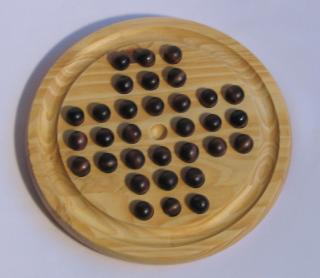
\includegraphics[height=2.5in, width=3.5in]{figs/PegSolitaire_full.jpg}
\caption{Full but the center case}
\label{fig_full}
\end{figure}
And the result for our different methods are as shown in table \ref{tab_resfull}:
\begin{table}[h!]
  \centering
  \begin{tabular}{ | c | c |  c | c | c | c |  c | c| c|}
\hline
case/\#nodeExpand & ID-DFS & $A*- 1$ & $A*-2$ & $A*-3$ & $A*-4$ & $A*-Manhattan$ & $A*-mix$ & Baseline \\ \hline
Extreme & MemErr & 1,967,299 & 175 & 5,714,286 & 530,537 & 1,801,655 & 103,402 & 26,847 \\ \hline
  \end{tabular}
  \caption{This table shows some data}
  \label{tab_resfull}
\end{table}
\subsection {Mean and Median}
For the whole benchmark, we calculated the mean and the median numbers of the expanded nodes in table \ref{tbl_mean}. In comparison we chose $A*-1$ and $A*-mix24"$ in our final submitted program. \\
\begin{table}[h!]
  \centering
  \begin{tabular}{ | c | c |  c | c | c | c |  c | c| c|}
\hline
\#nodeExpand & ID-DFS & $A*- 1$ & $A*-2$ & $A*-3$ & $A*-4$ & $A*-Manhattan$ & $A*-mix$ & Baseline \\ \hline
Mean & 1,979,736, & 47,084 & 4,398 & 46,408 & 8,937 & 19,201 & 3,388 & 5,146 \\ \hline
Median & 6,417 & 74 & 129 & 74 & 114 & 95 & 98 & 92 \\ \hline
  \end{tabular}
  \caption{This table shows some data}
  \label{tbl_mean}
\end{table}

\subsection {Performance Study with other tricks}
In our testing, we found one interesting phenomenon. For several large cases, if the movement orders are different, for example, expand one node by the order "East, West, North, South" might be quite different from the order "East, North, West, South". \\
There are 24 possible orders, where $24 = 4!$, and we tested all the 24 possible orders with the above 6 methods, which included five A* methods and one baseline method. And we counted two sets of summations, one is the set of summations for "opposite-order first" for the movements and another set of summations is for the "non-opposite-order first". Here "opposite-order first" contained 12 conditions starting with opposite directions at the first two and the last two pairs such as "East, West, North, South". For "non-opposite-order first", such as "East, North, West, South". In a box plot in figure \ref{fig_boxplot}, it's obvious that the "non-opposite-order first" had better.
\begin{figure} [h!]
\centering
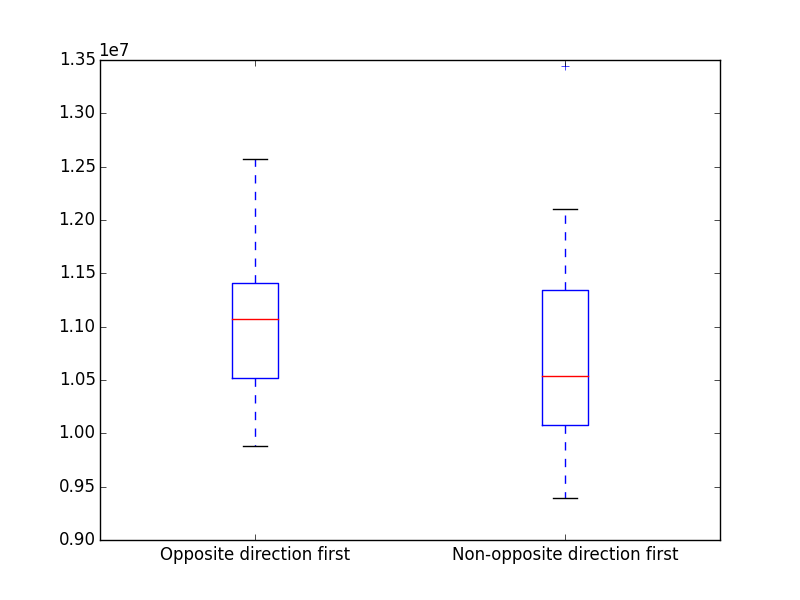
\includegraphics[height=3.5in, width=4.5in]{figs/boxplot.png}
\caption{Box plot for two sets of summations}
\label{fig_boxplot}
\end{figure}

\section {Conclusion}

\end{document}
